%%%%%%%%%%%%%%%%%%%%%%%%%%%%%%%%%%%%%%%%%%%%%%%%%%%%%%%%%%%%%%%%%%%%%%%%%%%%%%%%%%%%%%%%%%%%%%%%
%
% CSCI 1430 Written Question Template
%
% This is a LaTeX document. LaTeX is a markup language for producing documents.
% Your task is to answer the questions by filling out this document, then to
% compile this into a PDF document.
%
% TO COMPILE:
% > pdflatex thisfile.tex

% If you do not have LaTeX, your options are:
% - VSCode extension: https://marketplace.visualstudio.com/items?itemName=James-Yu.latex-workshop
% - Online Tool: https://www.overleaf.com/ - most LaTeX packages are pre-installed here (e.g., \usepackage{}).
% - Personal laptops (all common OS): http://www.latex-project.org/get/ 
%
% If you need help with LaTeX, please come to office hours.
% Or, there is plenty of help online:
% https://en.wikibooks.org/wiki/LaTeX
%
% Good luck!
% The CSCI 1430 staff
%
%%%%%%%%%%%%%%%%%%%%%%%%%%%%%%%%%%%%%%%%%%%%%%%%%%%%%%%%%%%%%%%%%%%%%%%%%%%%%%%%%%%%%%%%%%%%%%%%
%
% How to include two graphics on the same line:
%
% \includegraphics[width=0.49\linewidth]{yourgraphic1.png}
% \includegraphics[width=0.49\linewidth]{yourgraphic2.png}
%
% How to include equations:
%
% \begin{equation}
% y = mx+c
% \end{equation}
%
%%%%%%%%%%%%%%%%%%%%%%%%%%%%%%%%%%%%%%%%%%%%%%%%%%%%%%%%%%%%%%%%%%%%%%%%%%%%%%%%%%%%%%%%%%%%%%%%

\documentclass[11pt]{article}

\usepackage[english]{babel}
\usepackage[utf8]{inputenc}
\usepackage{amssymb}
\usepackage{xcolor}
\usepackage[colorlinks = true,
            linkcolor = blue,
            urlcolor  = blue]{hyperref}
\usepackage[a4paper,margin=1.5in]{geometry}
\usepackage{stackengine,graphicx}
\usepackage{fancyhdr}
\setlength{\headheight}{15pt}
\usepackage{microtype}
\usepackage{times}
\usepackage[shortlabels]{enumitem}
\setlist[enumerate]{topsep=0pt,itemsep=2pt,parsep=2pt}
\usepackage{amsmath}
\usepackage{framed}
\usepackage{mdframed}
\usepackage{xcolor}
\usepackage[most]{tcolorbox}
\usepackage{booktabs}

% a great python code format: https://github.com/olivierverdier/python-latex-highlighting
\usepackage{pythonhighlight}

\usepackage{trimclip,lipsum}

\frenchspacing
\setlength{\parindent}{0cm} % Default is 15pt.
\setlength{\parskip}{0.3cm plus1mm minus1mm}

\pagestyle{fancy}
\fancyhf{}
\lhead{Homework 5 Written Questions}
\rhead{CSCI 1430}
\lfoot{\textcolor{red}{\textbf{Only}
\ifcase\thepage
\or \textbf{instructions}
\or \textbf{Q1 (a)}
\or \textbf{Q1 (b)}
\or \textbf{Q2}
\or \textbf{Q3 (a) - (b)}
\or \textbf{Q3 (c)}
\or \textbf{Q4 (a) - (b)}
\or \textbf{Q4 (c) - (e)}
\or \textbf{Q4 (f) - (g)}
\or \textbf{Q5 (a)}
\or \textbf{Q5 (b)}
\or \textbf{Q6}
\or \textbf{Q6}
\or \textbf{Q6}
\or \textbf{Q6}
\or \textbf{feedback}
\else
\textbf{[ERROR: PAGE MISALIGNMENT]}
\fi
\textbf{should be on this page}
}}
\rfoot{\thepage~/ 16}


\date{}

\title{Homework 5 Written Questions}


\begin{document}
\maketitle
\thispagestyle{fancy}

\section*{Template Instructions}

This document is a template with specific answer regions and a fixed number of pages. Given large class sizes and limited TA time, the template helps the course staff to grade efficiently and still focus on the content of your submissions. Please help us in this task:
 
\begin{itemize}
  \item Make this document anonymous.
  
  \item Questions are in the orange boxes. Provide answers in the green boxes.
  \item Use the footer to check for correct page alignment.

  \item \textbf{Do NOT remove the answer box.}
  \item \textbf{Do NOT change the size of the answer box.}
  \item \textbf{Extra pages are not permitted unless otherwise specified.}
  \item \textbf{Template edits or page misalignment will lead to a 10 point deduction.}
\end{itemize}

\section*{Gradescope Submission}
\begin{itemize}
  \item Compile this document to a PDF and submit it to Gradescope.
  \item Pages will be automatically assigned to the right questions on Gradescope.
\end{itemize}

\section*{This Homework}
\begin{itemize}
    \item 5 questions \textbf{[8 + 6 + 6 + 10 + 12 = 42 points]}.
    \item 1 extra credit question \textbf{[10 points]} (good for capstone).
    \item Include code, images, and equations where appropriate.
\end{itemize}

\pagebreak

%%%%%%%%%%%%%%%%%%%%%%%%%%%%%%%%%%%
\paragraph{Q1:} \textbf{[8 points]} Many traditional computer vision algorithms use convolutional filters to extract feature representations, e.g., in SIFT, to which we then often apply machine learning classification techniques. Convolutional neural networks also use filters within a machine learning algorithm.

\begin{enumerate} [(a)]
\item \textbf{[4 points]}

\begin{tcolorbox}[colback=orange!5!white,colframe=orange!75!black]
What is different about the construction of the filters in each of these approaches? \textbf{[3--4 sentences]}
\end{tcolorbox}
\begin{tcolorbox}[colback=white!5!white,colframe=green!75!black]
    \setbox0=\hbox{\parbox[t]{\textwidth}{
    %%%%%%% ANSWER STARTS HERE %%%%%%%%%%%%%%%%%%%%%%%%%%%%
    
    TODO: Your answer for (a) here
    %%%%%% Remove this line in your answer! %%%%%%
    
    %%%%%%% ANSWER ENDS HERE %%%%%%%%%%%%%%%%%%%%%%%%%%%%%%
    }}
    \clipbox{0pt \dimexpr\dp0-16\baselineskip\relax{} 0in 0pt}{\copy0}
\end{tcolorbox}

\pagebreak
\item \textbf{[4 points]}
\begin{tcolorbox}[colback=orange!5!white,colframe=orange!75!black]
Please declare and explain at least two advantages and disadvantages of each of these two approaches (four total). \textbf{[6--8 sentences]}
\end{tcolorbox}
\begin{tcolorbox}[colback=white!5!white,colframe=green!75!black]
    \setbox0=\hbox{\parbox[t]{\textwidth}{
    %%%%%%% ANSWER STARTS HERE %%%%%%%%%%%%%%%%%%%%%%%%%%%%
    
    TODO: Your answer for (b) here 
    %%%%%% Remove this line in your answer! %%%%%%
    
    %%%%%%% ANSWER ENDS HERE %%%%%%%%%%%%%%%%%%%%%%%%%%%%%%
    }}
    \clipbox{0pt \dimexpr\dp0-16\baselineskip\relax{} 0in 0pt}{\copy0}
\end{tcolorbox}
\end{enumerate}


%%%%%%%%%%%%%%%%%%%%%%%%%%%%%%%%%%%
\pagebreak
\paragraph{Q2:} \textbf{[6 points]} Many CNNs have a multi-layer perceptron (MLP) after the convolutional layers as a general purpose decision-making subnetwork. The MLP is constructed from `dense' or `fully-connected' layers. In these, every output perceptron is connected to every input. This contrasts with convolutional layers, where each kernel operates on local windows of the previous layer activations.

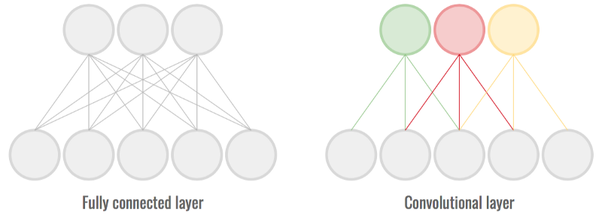
\includegraphics[width=\linewidth]{images/q2mlp.png}

Suppose we imagine a `locally-connected MLP', where every output perceptron is only connected to a small subset of nearby inputs.

\begin{tcolorbox}[colback=orange!5!white,colframe=orange!75!black]
Describe three differences that might occur when using a \emph{locally-connected} MLP versus a \emph{fully-connected} MLP, and explain why.
This might be in terms of the network's performance, its behavior on different data, the learned convolution kernel or perceptron weights, the optimization process, etc. \textbf{[6--9 sentences]}
\end{tcolorbox}

\begin{tcolorbox}[colback=white!5!white,colframe=green!75!black]
    \setbox0=\hbox{\parbox[t]{\textwidth}{
    %%%%%%% ANSWER STARTS HERE %%%%%%%%%%%%%%%%%%%%%%%%%%%%
    
    TODO: Your answer here 
    %%%%%% Remove this line in your answer! %%%%%%
    
    %%%%%%% ANSWER ENDS HERE %%%%%%%%%%%%%%%%%%%%%%%%%%%%%%
    }}
    \clipbox{0pt \dimexpr\dp0-18\baselineskip\relax{} 0in 0pt}{\copy0}
\end{tcolorbox}


\pagebreak
\paragraph{Q3:} \textbf{[6 points]} 
\begin{tcolorbox}[colback=orange!5!white,colframe=orange!75!black]
Given a neural network classifier and the stochastic gradient descent training scheme, discuss how the following hyperparameters might affect the training process and outcome.
\end{tcolorbox}

\begin{enumerate}[(a)]
    \item \textbf{[2 points]} Learning rate \textbf{[2--3 sentences]}
    \begin{tcolorbox}[colback=white!5!white,colframe=green!75!black]
    \setbox0=\hbox{\parbox[t]{\textwidth}{
    %%%%%%% ANSWER STARTS HERE %%%%%%%%%%%%%%%%%%%%%%%%%%%%
    
    TODO: Your answer for (a) here 
    %%%%%% Remove this line in your answer! %%%%%%
    
    %%%%%%% ANSWER ENDS HERE %%%%%%%%%%%%%%%%%%%%%%%%%%%%%%
    }}
    \clipbox{0pt \dimexpr\dp0-12\baselineskip\relax{} 0in 0pt}{\copy0}
    \end{tcolorbox}
    \item \textbf{[2 points]} Batch size \textbf{[2--3 sentences]}
    \begin{tcolorbox}[colback=white!5!white,colframe=green!75!black]
    \setbox0=\hbox{\parbox[t]{\textwidth}{
    %%%%%%% ANSWER STARTS HERE %%%%%%%%%%%%%%%%%%%%%%%%%%%%
    
    TODO: Your answer for (b) here 
    %%%%%% Remove this line in your answer! %%%%%%
    
    %%%%%%% ANSWER ENDS HERE %%%%%%%%%%%%%%%%%%%%%%%%%%%%%%
    }}
    \clipbox{0pt \dimexpr\dp0-12\baselineskip\relax{} 0in 0pt}{\copy0}
    \end{tcolorbox}

    \pagebreak
    \item \textbf{[2 points]} Number of epochs  \textbf{[2--3 sentences]}
    \begin{tcolorbox}[colback=white!5!white,colframe=green!75!black]
    \setbox0=\hbox{\parbox[t]{\textwidth}{
    %%%%%%% ANSWER STARTS HERE %%%%%%%%%%%%%%%%%%%%%%%%%%%%
    
    TODO: Your answer for (c) here 
    %%%%%% Remove this line in your answer! %%%%%%
    
    %%%%%%% ANSWER ENDS HERE %%%%%%%%%%%%%%%%%%%%%%%%%%%%%%
    }}
    \clipbox{0pt \dimexpr\dp0-12\baselineskip\relax{} 0in 0pt}{\copy0}
    \end{tcolorbox}
\end{enumerate}

\pagebreak
\paragraph{Q4:} \textbf{[10 points]} What effects are caused by adding a spatial max pooling layer (stride $>$ 1) between two convolutional layers, where the output with max pooling is some size larger than $1 \times 1 \times d$?

There may be multiple correct answers per question.

\emph{Tip:} To fill in boxes, replace `\textbackslash square' with `\textbackslash blacksquare' for your answer.

% \paragraph{A4:} Multiple choice. Choose all that apply.

%%% See the tex for the bottom of the page to leave the optional written justification %%%

\begin{enumerate}[(a)]
    \item \textbf{[1 point]}
    \begin{tcolorbox}[colback=orange!5!white,colframe=orange!75!black]
    What happens to the computational cost of training? (Ignore the cost of the max pooling layer itself.)
    \end{tcolorbox}
    \begin{tcolorbox}[colback=white!5!white,colframe=green!75!black]
    
    \begin{tabular}[h]{lr}
    \toprule
    Increases & $\square$ \\
    Stays the same & $\square$ \\
    Decreases & $\square$ \\
    \bottomrule
    \end{tabular}
    \end{tcolorbox}
    
    \item \textbf{[1 point]}
    \begin{tcolorbox}[colback=orange!5!white,colframe=orange!75!black]
    What happens to the computational cost of testing? (Ignore the cost of the max pooling layer itself.)
    \end{tcolorbox}
    \begin{tcolorbox}[colback=white!5!white,colframe=green!75!black]

    \begin{tabular}[h]{lr}
    \toprule
    Increases & $\square$ \\
    Stays the same & $\square$ \\
    Decreases & $\square$ \\
    \bottomrule
    \end{tabular}
    \end{tcolorbox}

\pagebreak
    \item \textbf{[1 point]}
    \begin{tcolorbox}[colback=orange!5!white,colframe=orange!75!black]
    What happens to the complexity of the decision function?
    \end{tcolorbox}
    \begin{tcolorbox}[colback=white!5!white,colframe=green!75!black]
    TODO: Select the right option %%%%%% Remove this line in your answer! %%%%%%

    \begin{tabular}[h]{lr}
    \toprule
    Increases & $\square$ \\
    Stays the same & $\square$ \\
    Decreases & $\square$ \\
    \bottomrule
    \end{tabular}
    \end{tcolorbox}

    \item \textbf{[1 point]}
    \begin{tcolorbox}[colback=orange!5!white,colframe=orange!75!black]
    What happens to the potential for overfitting?
    \end{tcolorbox}
    \begin{tcolorbox}[colback=white!5!white,colframe=green!75!black]

    \begin{tabular}[h]{lr}
    \toprule
    Increases & $\square$ \\
    Stays the same & $\square$ \\
    Decreases & $\square$ \\
    \bottomrule
    \end{tabular}
    \end{tcolorbox}

    \item \textbf{[1 point]}
    \begin{tcolorbox}[colback=orange!5!white,colframe=orange!75!black]
    What happens to the potential for underfitting?
    \end{tcolorbox}
    \begin{tcolorbox}[colback=white!5!white,colframe=green!75!black]
    
    \begin{tabular}[h]{lr}
    \toprule
    Increases & $\square$ \\
    Stays the same & $\square$ \\
    Decreases & $\square$ \\
    \bottomrule
    \end{tabular}
    \end{tcolorbox}

\pagebreak
    \item \textbf{[3 point]}
    In computer vision, we often care about producing invariant (or equivariant) representations. For instance, convolution is `translation equivariant' because a translation of the input induces a translation of the output. CNNs attempt to exploit this property to detect objects at any position in the image.

    \begin{tcolorbox}[colback=orange!5!white,colframe=orange!75!black]
    Which of the following does max pooling provide?
    \end{tcolorbox}

    \emph{Here,} `global' = the whole image, and `local' = only within the pooling region.

    \begin{tcolorbox}[colback=white!5!white,colframe=green!75!black]
    \begin{tabular}[h]{lr}
    \toprule
    Provides local rotational invariance & $\square$ \\
    Provides global rotational invariance & $\square$ \\
    Provides local scale invariance & $\square$ \\
    Provides global scale invariance & $\square$ \\
    Provides local translational invariance & $\square$ \\
    Provides global translational invariance & $\square$ \\
    \bottomrule
    \end{tabular}
    \end{tcolorbox}

    \item \textbf{[2 point]}
    \begin{tcolorbox}[colback=orange!5!white,colframe=orange!75!black]
    In a CNN, is the convolutional property of translation equivariance maintained through max pooling? Why or why not?
    
    \vspace{1em}
    \emph{Another way to think about it:} Suppose I was classifying birds. If a bird translates within the image frame but remains otherwise identical, will I still receive the same confidence of bird class?

    \vspace{1em}
    \emph{Note:} It might help to relate different pooling functions to downsampling, and to consider what we know about downsampling, image frequency, and aliasing.
    \textbf{[4--6 sentences]}
    \end{tcolorbox}

    \begin{tcolorbox}[colback=white!5!white,colframe=green!75!black]
    \setbox0=\hbox{\parbox[t]{\textwidth}{
    %%%%%%% ANSWER STARTS HERE %%%%%%%%%%%%%%%%%%%%%%%%%%%%
    
    TODO: Your answer for (g) here 
    %%%%%% Remove this line in your answer! %%%%%%
    
    %%%%%%% ANSWER ENDS HERE %%%%%%%%%%%%%%%%%%%%%%%%%%%%%%
    }}\clipbox{0pt \dimexpr\dp0-13\baselineskip\relax{} 0in 0pt}{\copy0}
    \end{tcolorbox}

\end{enumerate}


\pagebreak

\paragraph{Q5 (a):} \textbf{[6 points]} Stakeholders of automated decision-making systems often require explanations for the system's decisions. In some situations, there exists a \href{https://en.wikipedia.org/wiki/Right_to_explanation}{right to explanation}; the US Government's \href{https://www.whitehouse.gov/ostp/ai-bill-of-rights/}{Blueprint for an AI Bill of Rights} includes such a right. But, the benefits of a technology may exist even if an explanation for its mechanism is unknown; the mechanism for the painkiller and anti-inflamatory drug \emph{aspirin}, in wide use since the early 20th century, was only \href{https://en.wikipedia.org/wiki/History_of_aspirin#Investigating_how_aspirin_works}{correctly identified in the 1970s}.

For example, in medical imaging, hand designed features from biological experts might lead to explainable methods for patients, physicians, and regulators. However, deep learning methods can show \href{https://drive.google.com/file/d/1bDAqEtW482OJeqMBt5A4AradVa4gf_o9/view}{higher test accuracy}, even if interpreting their `black box' nature to explain their decisions remains an open question.

For your final project, you create a CNN to diagnose skin cancer from skin lesion images in the \href{https://challenge2020.isic-archive.com/}{International Skin Imaging Collaboration (ISIC) dataset}. In testing, you find that your CNN can detect this disease with 90\% accuracy. Prior technology can detect this disease with only 60\% accuracy. You have no medical qualification. You cannot explain how your CNN accurately detects the disease so accurately, just that it does.

\begin{tcolorbox}[colback=orange!5!white,colframe=orange!75!black]
    Suppose you were asked by Rhode Island Hospital to consider using this model in a clinical setting. Describe three factors or assessments that would make you more or less confident in its use and explain why. \textbf{[6--9 sentences]}
\end{tcolorbox}

\begin{tcolorbox}[colback=white!5!white,colframe=green!75!black]
\setbox0=\hbox{\parbox[t]{\textwidth}{
%%%%%%% ANSWER STARTS HERE %%%%%%%%%%%%%%%%%%%%%%%%%%%%

TODO: Your answer here %%%%%% Remove this line in your answer! %%%%%%

%%%%%%% ANSWER ENDS HERE %%%%%%%%%%%%%%%%%%%%%%%%%%%%%%
}}
\clipbox{0pt \dimexpr\dp0-22\baselineskip\relax{} 0in 0pt}{\copy0}
\end{tcolorbox}


%%%%%%%%%%%%%%%%%%%%%%%%%%%%%%%%%%%
\pagebreak 
\paragraph{Q5 (b):} \textbf{[6 points]} There are many attempts to explain CNN predictions; we refer the interested reader to \href{https://christophm.github.io/interpretable-ml-book/}{Christoph Molar's Interpretable ML Book}. Let's consider three:
\begin{enumerate}
    \item In class, we saw \href{https://adamharley.com/nn_vis/cnn/2d.html}{Adam Harley's neural network visualizer}, which visualizes how a CNN predicts numerals when trained on the MNIST dataset.
    
    \item In the code, we will use \href{https://christophm.github.io/interpretable-ml-book/lime.html#example-7}{Local Interpretable Model-agnostic Explanations (LIME)} to attempt to explain model predictions. LIME assesses which image superpixels are important to a classification, independent of any inner workings of the model.

    \item Saliency maps attempt to show which image pixels are sensitive to the classification via the dependence on the inner working of the model via its gradients. 
    Please read \href{https://christophm.github.io/interpretable-ml-book/pixel-attribution.html#examples-6}{Sections 10.2.6--10.2.9} for examples and analysis. 
\end{enumerate}

In the ISIC dataset, it was found that ``half of the images of benign lesions contain elliptical coloured patches (colour calibration charts), whereas the malignant lesion images contain none'' (\href{https://www.mdpi.com/2075-4418/12/1/40}{Nauta et al.}, see Figure 1 for patch examples) and that imaging rulers and standard surgical ink markers were unevenly distributed in the data. These can lead to \emph{spurious correlations} in training where unimportant image features are associated to classification outcomes. \href{https://www.ncbi.nlm.nih.gov/pmc/articles/PMC6694463/}{Winkler et al.} found that the presence of ink markings led to a 40\% increase in false positive rate (see Figure 1 for ink marking examples).


\begin{tcolorbox}[colback=orange!5!white,colframe=orange!75!black]
To what extent would each of these interpretability methods improve your understanding of your medical imaging CNN's predictions, and why?
To what extend would each of these interpretability methods help explain the CNNs decision to a patient?
\textbf{[6--9 sentences]}
\end{tcolorbox}

\begin{tcolorbox}[colback=white!5!white,colframe=green!75!black]
\setbox0=\hbox{\parbox[t]{\textwidth}{
%%%%%%% ANSWER STARTS HERE %%%%%%%%%%%%%%%%%%%%%%%%%%%%

TODO: Your answer here %%%%%% Remove this line in your answer! %%%%%%

%%%%%%% ANSWER ENDS HERE %%%%%%%%%%%%%%%%%%%%%%%%%%%%%%
}}
\clipbox{0pt \dimexpr\dp0-19\baselineskip\relax{} 0in 0pt}{\copy0}
\end{tcolorbox}


% Please leave the pagebreak
\pagebreak
%%%%%%%%%%%%%%%%%%%%%%%%%%%%%%%%%%%%%
\textbf{Q6:} Two important notes:

\begin{enumerate}
\item \emph{The next question is extra credit, worth up to 10 pts}. If you are capstoning the class, this can also count as your required extra credit attempt for HW5; none further in the code is required.

\item The next question provides details for how we construct simple neural networks from scratch with sigmoid and softmax activations. Then, it asks you to map this to Python by filling in gaps in functions given in stencil code. \emph{It is longer and more involved, in tutorial style, and requires careful reading.} If you want insight from implementing a simple neural network, then this is the question to answer.
\end{enumerate}

\paragraph{Q6 Background:}
Let us consider using a neural network (non-convolutional) to perform classification on the \href{http://yann.lecun.com/exdb/mnist/}{MNIST dataset} of handwritten digits, with 10 classes covering the digits 0--9. Each database image is 28$\times$28 pixels, and comes with a label as supervision denoting the image's class $\mathbf{y}=(y_1,y_2,\dots,y_i,\dots,y_{10})$. As our image is 28$\times$28, the network input is a linearization of each image into a 784-dimensional vector $\mathbf{x}=(x_1,x_2,\dots,x_i,\dots,x_{784})$. The output of the neural network is a probability distribution $\mathbf{p}=(p_1,\dots,p_j,\dots,p_{10})$ over the 10 classes. Suppose our network has one fully-connected layer with $10$ neurons---one for each class. Each neuron has a weight for each input $\mathbf{w}=(w_1,\dots,w_i,\dots,w_{784})$, plus a bias $b$. As we only have one layer with no multi-layer composition, there's no need to use an activation function.

When we pass in a vector $\mathbf{x}$ to this layer, we will compute a 10-dimensional output vector $\mathbf{l}=(l_1,l_2,...,l_j,...,l_{10})$ as:
\begin{equation}
    l_j = \mathbf{w}_j \cdot \mathbf{x} + b_j = \sum_{i=1}^{784}w_{ij}x_i + b_j
\end{equation}
These distances from the hyperplane are sometimes called `logits' (hence $l$) when they are the output of the last layer of a network. In our case, we only have \emph{one} layer, so our single layer is the last layer.

\hspace{\fill}\rule{0.5\linewidth}{.5pt}\hspace{\fill}

Often we want to talk about the confidence of a classification. So, to turn our logits into a probability distribution $\mathbf{p}$ for our ten classes, we apply the \emph{softmax} function:
\begin{equation}
    p_j = \frac{e^{l_j}}{\sum_je^{l_j}}
    \label{eq:softmax}
\end{equation}
Each $p_j$ will be positive, and $\sum_jp_j = 1$, and so softmax is guaranteed to output a probability distribution. Picking the most probable class provides our network's prediction.

\emph{If} our weights and biases were optimized, Eq.~\ref{eq:softmax} would classify a new test example.

\hspace{\fill}\rule{0.5\linewidth}{.5pt}\hspace{\fill}

We have two probability distributions: the true distribution of answers from our training labels $\mathbf{y}$, and the predicted distribution produced by our current classifier $\mathbf{p}$. To train our network, our goal is to define a loss to reduce the distance between these distributions.

Let $y_j=1$ if class $j$ is the true label for $x$, and $y_j = 0$ if $j$ is not the true label. Then, we define the \emph{cross-entropy loss}:
\begin{equation}
    L(w,b,x) = - \sum_{j=1}^{10}y_j\ln(p_j),
\end{equation}
which, after substitution of Eqs. 2 and 1, lets us compute an error (remember that: error = 1 - accuracy) between the labeled ground truth distribution and our predicted distribution.

So...why does this loss $L$ work? Using the cross-entropy loss exploits concepts from information theory---Aur\'{e}lien G\'{e}ron has produced \href{https://www.youtube.com/watch?v=ErfnhcEV1O8}{a video with a succinct explanation of this loss}. Briefly, the loss minimizes the difference in the amounts of information needed to represent the labeled ground truth distribution and our predicted distribution---when the amount of information needed is similar, both distributions are similar, and our neural network predicts the correct labels for the input images. Other losses are applicable, with their own interpretations, but these details are beyond the scope of this course.

%%%%%%%%%%%%%%%%%%%
% Cheat sheet for information theory
%
% Probability distribution \mathbf{p}
% Describes the likelihood of different outcomes, e.g., suppose our MNIST dataset samples are each of a class '0,1,2,3,4,5,6,7,8,9' with non-uniform data distribution. We might have a 0.09 chance that an image will be of a character '0', 0.11 for a '1', 0.08 for a '2', and so on, with the sum chances for all characters being 1.0.
%
% What is entropy?  H(\mathbf{p}) = - \sum_{i} p_i \log{p_i}
% Probability of an event multiplied by the reduction in uncertainty (or amount of information) received from that event. Is the average amount of information (in bits) that we receive from one sample drawn from a probability distribution. It tells us how predictable that probability distribution is (or, written another way, how uncertain we are). 0 entropy = no uncertainty. High entropy = very uncertain probability distribution.
%
% What is cross-entropy?   H(\mathbf{p},\mathbf{q}) = - \sum_{i} p_i \log_2{q_i}
% The average message length in bits _across_ two distributions - e.g., the true distribution \mathbf{p} and some _predicted_ distribution \mathbf{q}. If the predicted distribution is equal to the true distribution, then cross-entropy _is_ entropy.
%
% So then what is entropy minus cross-entropy?
% This tells us how different the predicted distribution is from the true distribution. This is called the Kullback-Leibler divergence (or KL-divergence). It is a divergence and not a distance because it doesn't have a `sidedness'.
% D_{KL}(\mathbf{p} || \mathbf{q}) = H(\mathbf{p},\mathbf{q}) - H(\mathbf{p})
%
% Why is it \emph{minus}?   
% The uncertainty reduction factor from a message is equal to 1 / p(event). So, we would normally compute log( 1/p(event) ). But log(1/x) = -log(x), so we equivalently compute -log( p(event) ).
%
%%%%%%%%%%%%%%%%%%%

\hspace{\fill}\rule{0.5\linewidth}{.5pt}\hspace{\fill}

Onto the training algorithm. The loss is computed once for every different training example. When every training example has been presented, we call this an \emph{epoch}. We will train for many epochs until our loss over all training examples is minimized.

Neural networks are usually optimized using gradient descent. For each training example in each epoch, we compute gradients via backpropagation (an application of the chain rule in differentiation) to update the classifier parameters $w_{ij}, b_j$ via a learning rate $\lambda$:
\begin{equation}
w_{ij} = w_{ij} - \lambda\frac{\partial L}{\partial w_{ij}}, \\
\label{eq:graddesc_updateweights}
\end{equation}
\begin{equation}
b_j = b_j - \lambda\frac{\partial L}{\partial b_j}.
\label{eq:graddesc_updatebias}
\end{equation}

To update the weights and bias with gradient descent via Eqs.~\ref{eq:graddesc_updateweights} and \ref{eq:graddesc_updatebias}, we must deduce $\frac{\partial L}{\partial w_{ij}}$ and $\frac{\partial L}{\partial b_j}$ as expressions in terms of $x_i$ and $p_j$.

\emph{Intuition:} Let's just consider the weights for now. Recall that our network has one layer of neurons followed by a softmax function. To compute the change in the cross-entropy loss $L$ with respect to neuron weights $\frac{\partial L}{\partial w_{ij}}$, we will need to compute and chain together three different terms:
\begin{enumerate}
\itemsep0em
\listparindent0em
\topsep0em
\parsep0em
\partopsep0em
\item The change in the loss with respect to the softmax output $\frac{\delta L}{\delta p_j}$,
\item The change in the softmax output with respect to the neuron output $\frac{\delta p_j}{\delta l_j}$, and
\item The change in the neuron output with respect to the neuron weights $\frac{\delta l_j}{w_{ij}}$.
\end{enumerate}
We must derive each individually, and then formulate the final term via the chain rule. The biases follow in a similar fashion.

The derivation is beyond the scope of this class, and so we provide them here:
\begin{equation}
\frac{\delta L}{\delta w_{ij}} = \frac{\delta L}{\delta p_a} \frac{\delta p_a}{\delta l_j} \frac{\delta l_j}{\delta w_{ij}} =\begin{cases}
x_i(p_j-1), a = j\\
x_ip_j,  a\neq j
\end{cases}
\label{eq:wupdate}
\end{equation}
\begin{equation}
\frac{\delta L}{\delta b_j} = \frac{\delta L}{\delta p_a} \frac{\delta p_a}{\delta l_j} \frac{\delta l_j}{\delta b_j} =\begin{cases}
(p_j-1), a = j\\
p_j,  a\neq j
\end{cases}
\label{eq:bupdate}
\end{equation}
Here, $a$ is the predicted class label and $j$ is the true class label. An alternative form you might see shows $\frac{\delta L}{\delta w_{ij}} = x_i(p_j-y_j)$ and $\frac{\delta L}{\delta b_j} = p_j-y_j$ where $y_j=1$ if class $j$ is the true label for $x$, and $y_j = 0$ if $j$ is not the true label.

So...after all of that, our gradient update rules are surprisingly simple!

\emph{Further details:} For interested students, we refer students to Chapter 1 of \href{https://cs.brown.edu/courses/csci1460/assets/files/deep-learning.pdf}{Prof.~Charniak's deep learning notes}, which derives these gradient update rules. We also refer to \href{http://web.khu.ac.kr/~tskim/MLPR\%2025-3\%20Backpropagation%20with%20CE%20(Handout).pdf}{Prof.~Sadowski's notes on backpropagation}: Section 1 derives terms first for cross-entropy loss with logistic (sigmoid) activation, and then Section 2 derives terms for cross-entropy loss with softmax. The Wikipedia article on \href{https://en.wikipedia.org/wiki/Backpropagation}{the backpropagation algorithm} likewise represents a derivation walkthrough of the general case with many hidden layers each with sigmoid activation functions, and a final layer with a softmax function.

\hspace{\fill}\rule{0.5\linewidth}{.5pt}\hspace{\fill}


\paragraph{Q6:} We will implement these steps in code using numpy. We provide a code stencil \texttt{main.py} which loads one of two datasets: MNIST and the scene recognition dataset from Homework 4. We also provide two models: a neural network, and then a neural network whose logits are used as input to an SVM classifier. Please look at the comments in \texttt{main.py} for the arguments to pass in to the program for each condition. 

The neural network model is defined in \texttt{model.py}, and the parts we must implement are marked with TODO comments. Each requires only a few lines of code at most:
\begin{enumerate}
    \item Initialize the weights and biases in \pyth{__init__()}
    \item Complete the overall training flow in \pyth{train_nn()}
    \item Define the forward pass in \pyth{forward_pass()}
    \item Define the gradient descent update in \pyth{gradient_descent()}
    \item Define the cross-entropy loss in \pyth{loss()}
    \item Define the back-propagation rule in \pyth{back_propagation()}
\end{enumerate}

\begin{tcolorbox}[colback=orange!5!white,colframe=orange!75!black]
\emph{Tasks:} Implement the neural network and its optimization. \textbf{[10 points]}

\vspace{1em}
Please upload your completed \texttt{model.py} to Gradescope under the assignment titled ``Homework 5 Written (Numpy)''. The autograder will check that you correctly implemented parts of your model. Then, report your accuracy here.
\end{tcolorbox}

\begin{tcolorbox}[colback=orange!5!white,colframe=orange!75!black]
Run your model on all four conditions and report training loss (calculated using \emph{training} set) and accuracy (calculated using \emph{testing} set) as the number of training epochs increases. Why does the SVM perform differently?
\end{tcolorbox}
\begin{tcolorbox}[colback=white!5!white,colframe=green!75!black]
\setbox0=\hbox{\parbox[t]{\textwidth}{
%%%%%%%%%%%%%%%%%%%%%%%%%%%%%%%%%%%%%%
% ANSWER STARTS HERE
% Replace all the 'xx's with your results
    \begin{itemize}
        \item NN on MNIST: xx\% (highest accuracy)
            \begin{itemize}
            \item Epoch 0 loss: xx     Accuracy: xx\%
            \item Epoch 9 loss: xx     Accuracy: xx\%
            \end{itemize}
        \item NN+SVM on MNIST: xx\% (highest accuracy)
            \begin{itemize}
            \item Epoch 0 loss: xx     Accuracy: xx\%
            \item Epoch 9 loss: xx     Accuracy: xx\%
            \end{itemize}
        \item NN on SceneRec: xx\% (highest accuracy)
            \begin{itemize}
            \item Epoch 0 loss: xx     Accuracy: xx\%
            \item Epoch 9 loss: xx     Accuracy: xx\%
            \end{itemize}
        \item NN+SVM on SceneRec: xx\% (highest accuracy)
            \begin{itemize}
            \item Epoch 0 loss: xx     Accuracy: xx\%
            \item Epoch 9 loss: xx     Accuracy: xx\%
            \end{itemize}
    \end{itemize}

\emph{Why does the SVM perform differently?}

TODO: Answer here
% ANSWER ENDS HERE
%%%%%%%%%%%%%%%%%%%%%%%%%%%%%%%%%%%%%%
}}
\clipbox{0pt \dimexpr\dp0-36\baselineskip\relax{} 0in 0pt}{\copy0}
\end{tcolorbox}


%%%%%%%%%%%%%%%%%%%%%%%%%%%%%%%%%%%
\pagebreak
\section*{Feedback? (Optional)}
Please help us make the course better. If you have any feedback for this assignment, we'd love to hear it!


% \pagebreak
% \section*{Any additional pages would go here.}


\end{document}
